%% Type de document et encodage de la police
\documentclass[a4paper]{article}
\usepackage[utf8]{inputenc}
\usepackage[T1]{fontenc}
\usepackage[colorlinks=true, allcolors=black]{hyperref}
% \usepackage[french]{babel}

%% Initialise la taille des pages et des marges
\usepackage[a4paper, top=3cm, bottom=3cm, left=2cm, right=2cm, marginparwidth=2cm]{geometry}

%% Packs utiles
\usepackage{amsmath}
\usepackage{graphicx}
\usepackage{pmboxdraw}

%% Commandes perso
\renewcommand{\arraystretch}{1.2} %% row 20% longer
\renewcommand{\contentsname}{Table des matières}

%% Pour les exemples
\usepackage{mdframed}
\newmdenv[topline=false, bottomline=false, rightline=false, skipabove=\topsep, skipbelow=\topsep]{example}

%% Pour les diagrammes
\usepackage{tikz}
\tikzstyle{incolore} = [rectangle, rounded corners, draw=black, minimum height=1cm, minimum width=3cm, text width=3cm, text centered]


\title{Sécurité des OS}
\author{Grégoire Roumache}
\date{Avril 2021}

\begin{document}

\maketitle \tableofcontents

\begin{center} \rule{0.99\linewidth}{0.2mm} \end{center}

\textbf{Remarques:}
\begin{itemize}
    \item j'ai regroupé la résolution des labos \textit{pfsense} avec ceux du cours de sécurité des réseaux
    \item je n'ai pas fait de synthèse zabbix
    \item les labos powershell sont traités dans la synthèse du cours de progra os
\end{itemize}















\section{Correction examen théorique de juin 2019}





\begin{enumerate}
    \item Que veut dire PAM ?
    \begin{enumerate}
        \item Pluggable Authentification Mechanism
        \item Pluggable Authorisation Mechanism
        \item \textcolor{blue}{\textbf{Pluggable Authentification Modules}}
        \item Pluggable Authorisation Modules
        \item Aucune de ces réponses
    \end{enumerate}
    \item Quel est le but de PAM ?
    \begin{enumerate}
        \item Centraliser l'authentification
        \item Fournir une API de développement de modules spécifiques d'authentification
        \item Permettre l'exécution de traitements spécifiques automatisés lors de l'authentification
        \item \textcolor{blue}{\textbf{Les réponses A, B, C sont toutes correctes}}
        \item Les réponses A, B, C ne sont pas toutes correctes
    \end{enumerate}
    \item Quel comportement engendre le contrôle \texttt{required} de PAM ?
    \begin{enumerate}
        \item \textcolor{blue}{\textbf{Tous les modules utilisant ce contrôle doivent passer avec succès pour que la vérification soit accordée. Le cas échéant l'utilisateur n'est averti qu'à la fin du traitement de la pile. Un échec empêche l'ouverture de session, les autres modules de la pile sont néanmoins exécutés.}}
        \item Tous les modules utilisant ce contrôle doivent passer avec succès pour que la vérification soit accordée. Le cas échéant l'utilisateur n'est averti qu'à la fin du traitement de la pile. Un échec empêche l'ouverture de session, les autres modules de la pile ne sont pas exécutés.
        \item Tous les modules utilisant ce contrôle doivent passer avec succès pour que la vérification soit accordée. Le cas échéant l'utilisateur est averti directement. Un échec empêche l'ouverture de session, les autres modules de la pile ne sont pas exécutés.
        \item Au moins un module utilisant ce contrôle doit passer avec succès pour que la vérification soit accordée. Le cas échéant l'utilisateur n'est averti qu'à la fin du traitement de la pile. Un échec empêche l'ouverture de session, les autres modules de la pile sont néanmoins exécutés.
        \item Au moins un module utilisant ce contrôle doit passer avec succès pour que la vérification soit accordée. Le cas échéant l'utilisateur est averti directement. Un échec empêche l'ouverture de session, les autres modules de la pile sont néanmoins exécutés.
    \end{enumerate}
    \item Sous PAM, quel groupe de gestion vérifie si le compte utilisateur est arrivé à expiration ?
    \begin{enumerate}
        \item session
        \item auth
        \item password
        \item \textcolor{blue}{\textbf{account}}
        \item Aucune de ces réponses
    \end{enumerate}
    \item Quel autre avantage est lié à l'utilisation de PAM ?
    \begin{enumerate}
        \item La possibilité d'utiliser la double authentification
        \item La possibilité de développer de nouveaux modules dans de multiples langages
        \item La possibilité d'utiliser PAM dans des environnements hétérogènes, sur des OS différents (Linux, Windows, MAC, ...)
        \item Les réponses A, B, C sont toutes correctes
        \item \textcolor{blue}{\textbf{Les réponses A, B, C ne sont pas toutes correctes}}
    \end{enumerate}
    \begin{example} Les réponses A et B sont correctes, pas la C. \end{example}
    \item Quelle action engendre le module \texttt{pam\_security.so} ?
    \begin{enumerate}
        \item Autorise le login par le compte root excepté sur les terminaux listés dans \texttt{/etc/securetty}
        \item Autorise le login par le compte root uniquement sur les terminaux listés dans \texttt{/etc/securetty}
        \item \textcolor{blue}{\textbf{Interdit le login par le compte root excepté sur les terminaux listés dans \texttt{/etc/securetty}}}
        \item Interdit le login par le compte root uniquement sur les terminaux listés dans \texttt{/etc/securetty}
        \item Aucune de ces réponses
    \end{enumerate}
    \item Quelle action engendre le module \texttt{pam\_cracklib.so} ?
    \begin{enumerate}
        \item S'assure que le mot de passe employé a été renouvelé dans les délais
        \item \textcolor{blue}{\textbf{S'assure que le mot de passe employé présente un niveau de sécurité suffisant}}
        \item S'assure que le mot de passe employé est présent dans le fichier \texttt{/etc/passwd}
        \item S'assure que le mot de passe employé n'a pas été corrompu
        \item Aucune de ces réponses
    \end{enumerate}
    \item Que veut dire LDAP ?
    \begin{enumerate}
        \item Lightweight Direct Access Protocol
        \item Lightweight Direct Authentification Protocol
        \item \textcolor{blue}{\textbf{Lightweight Directory Access Protocol}}
        \item Lightweight Directory Authentification Protocol
        \item Aucune de ces réponses
    \end{enumerate}
    \item LDAP est un protocole réseaux OSI de quelle couche ?
    \begin{enumerate}
        \item couche 2
        \item couche 3
        \item couche 4
        \item \textcolor{blue}{\textbf{couche 5}}
        \item couche 6
    \end{enumerate}
    \begin{example} 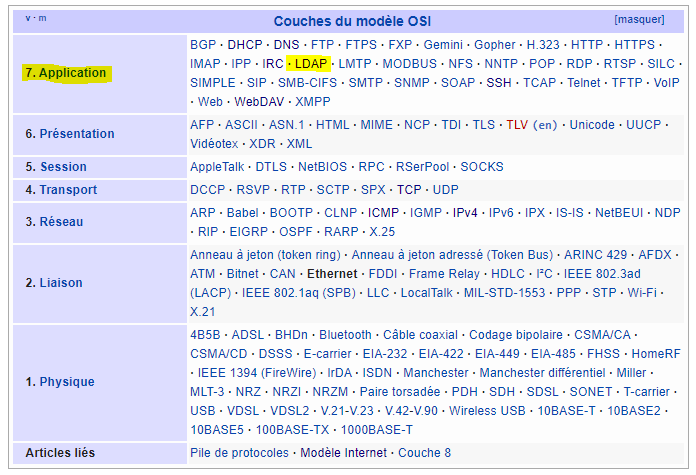
\includegraphics[width=0.75\linewidth]{images/OSI.PNG} \end{example}
    \item Pour établir une communication avec un serveur LDAP, le client doit obligatoirement fournir ?
    \begin{enumerate}
        \item \textcolor{blue}{\textbf{L'adresse IP + le numéro de port du serveur}}
        \item Un login et un mot de passe
        \item Le protocole d'authentification à utiliser
        \item Il doit fournir A + B + C (= les 3 réponses ci-dessus)
        \item Aucune de ces réponses
    \end{enumerate}
    \item Sous LDAP, qu'est ce que le DIT ?
    \begin{enumerate} 
        \item Le protocole réseau de communication
        \item Le protocole d'authentification choisi par le client
        \item \textcolor{blue}{\textbf{L'arbre d'information de l'annuaire}}
        \item Un noeud de la structure hiérarchique LDAP
        \item Aucune de ces réponses
    \end{enumerate}
    \begin{example} DIT = Directory Information Tree \end{example}
    \item Sous LDAP, qu'est-ce qu'un DN ?
    \begin{enumerate}
        \item Un nom distinctif qui compose le RDN
        \item \textcolor{blue}{\textbf{Un nom distinctif qui décrit une entrée de l'annuaire}}
        \item Un nom distinctif qui décrit la valeur d'une entrée
        \item Un nom distinctif qui décrit le type d'un attribut
        \item Aucune de ces réponses
    \end{enumerate}
    \begin{example} \begin{itemize}
        \item DN = Distinguished Name, nom absolu, unique, identifiant une entrée dans l'arborescence
        \item RDN = Relative Distinguished Name, nom d'un élément dans l'arborescence
        \item DN d'un élément = concaténation de l'ensemble des RDN de ses ascendants hiérarchiques
    \end{itemize} \end{example}
    \item Sous LDAP, pourquoi utiliser les classes ?
    \begin{enumerate}
        \item Pour regrouper des entrées possédant les mêmes valeurs
        \item Pour éviter d'avoir des entrées redondantes
        \item Pour regrouper des DN identiques
        \item \textcolor{blue}{\textbf{Pour éviter de définir plusieurs fois les attributs d'une entrée}}
        \item Aucune de ces réponses
    \end{enumerate}
    \item Sous LDAP, quelle opération n'est pas permise ?
    \begin{enumerate}
        \item Faire une recherche par critères
        \item Supprimer une entrée
        \item Modifier un DN
        \item Modifier une entrée
        \item \textcolor{blue}{\textbf{Toutes ces opérations sont permises}}
    \end{enumerate}
    \item Quel modèle ne fait pas partie des modèles LDAPv3 ?
    \begin{enumerate}
        \item Stockage d'informations
        \item Nommage
        \item Fonctionnel
        \item Sécurisation/confidentialité
        \item \textcolor{blue}{\textbf{Ce sont tous des modèles LDAPv3}}
    \end{enumerate}
    \item Le type de syntaxe d'un attribut LDAP défini...
    \begin{enumerate}
        \item Le type de donnée stockée (valeur)
        \item Le type de comportement lors d'une recherche
        \item Des contraintes sur les valeurs de l'attribut
        \item \textcolor{blue}{\textbf{Les réponses A, B, C sont correctes}}
        \item Aucune réponse n'est correcte
    \end{enumerate}
    \item Une classe utilisée comme modèle pour créer d'autres classes d'objets est appelée ?
    \begin{enumerate}
        \item Générique
        \item Structurelle
        \item \textcolor{blue}{\textbf{Abstraite}}
        \item Auxiliaire
        \item Globale
    \end{enumerate}
    \begin{example} \begin{itemize}
        \item abstraite = on peut l'instancier et la modifier comme on veut
        \item structurelle = nécessaire à la création
        \item auxiliaire = classe fourre-tout
    \end{itemize} \end{example}
    \item LDAP utilise les OIDs, qu'est-ce qu'un OID ?
    \begin{enumerate}
        \item Notation de synthèse abstraite qui définit les RDN
        \item \textcolor{blue}{\textbf{Chaine numérique qui identifie de façon unique un objet}}
        \item Notation de synthèse abstraite qui définit les attributs d'un objet
        \item Chaine numérique qui identifie de façon unique un serveur LDAP
        \item Globale
    \end{enumerate}
    \begin{example} OID = Object ID (= object identifier) \end{example}
    \item L'exemple suivant: \texttt{uid=john.doe,ou=People,dc=example,dc=com}, montre ?
    \begin{enumerate}
        \item \textcolor{blue}{\textbf{Un DN}}
        \item Un RDN
        \item Un OID
        \item Un UIT
        \item Un DIT
    \end{enumerate}
    \begin{example} UIT = /, sans doute une faute de frappe pour UID \end{example}
    \item LDIF est...
    \begin{enumerate}
        \item \textcolor{blue}{\textbf{Un format de fichier LDAP}}
        \item Un format de structure LDAP
        \item Un format de base de données LDAP
        \item Un format d'attribut LDAP
        \item Aucune réponse n'est correcte
    \end{enumerate}
    \begin{example} LDIP = LDAP Data Interchange Format, les données sont sous forme d'un fichier texte \end{example}
    \item Quelle fonctionnalité ne fait pas partie du modèle de sécurisation LDAP ?
    \begin{enumerate}
        \item Authentification
        \item Confidentialité
        \item Intégrité
        \item Autorisation
        \item \textcolor{blue}{\textbf{Aucune réponse n'est correcte}}
    \end{enumerate}
    \item PPP est un protocole d'authentification de ?
    \begin{enumerate}
        \item Couche 2
        \item Couche 3
        \item Couche 4
        \item Couche 5
        \item \textcolor{blue}{\textbf{Aucune réponse n'est correcte}}
    \end{enumerate}
    \item Quelle fonctionnalité supplémentaire MS-CHAPv2 apporte par rapport à MS-CHAPv1 ?
    \begin{enumerate}
        \item Le chiffrement du login
        \item Le chiffrement du mot de passe
        \item Le chiffrement du login et du mot de passe
        \item \textcolor{blue}{\textbf{L'authentification mutuelle}}
        \item Aucune réponse n'est correcte
    \end{enumerate}
    \item Quelle est la faille majeure de MS-CHAP ?
    \begin{enumerate}
        \item Le mot de passe est transmis non-chiffré
        \item \textcolor{blue}{\textbf{Le mot de passe est transmis chiffré mais il peut être déchiffré}}
        \item Il n'est pas compatible avec le protocole WPA2
        \item Le serveur utilise un port ouvert pour la réception des requêtes
        \item Aucune réponse n'est correcte
    \end{enumerate}
    \item PEAP est ?
    \begin{enumerate}
        \item Une méthode de chiffrement
        \item Un protocole d'échange de clé publique
        \item Un protocole d'authentification à 2 niveaux
        \item \textcolor{blue}{\textbf{Un protocole d'identification propriétaire Microsoft}}
        \item Aucune réponse n'est correcte
    \end{enumerate}
    \begin{example} PEAP = Protected Extensible Authentication Protocol \end{example}
    \item AAA: quelle réponse n'en fait pas partie ?
    \begin{enumerate}
        \item Authentification
        \item Gestion des autorisations
        \item Enregistrement de l'historique (log)
        \item \textcolor{blue}{\textbf{Contrôle de l'intégrité}}
        \item Aucune réponse n'est correcte
    \end{enumerate}
    \begin{example} Protocole AAA = Authentication, Authorization, Accounting/Auditing \end{example}
    \item À quoi correspond le x dans l'extension des fichiers scripts \texttt{powershell.psx} ?
    \begin{enumerate}
        \item Au niveau de la politique d'exécution du script
        \item \textcolor{blue}{\textbf{À la version de Powershell minimum compatible}}
        \item Au niveau de cryptage de la signature du script
        \item À la version de Powershell maximale compatible
        \item Aucune réponse n'est correcte
    \end{enumerate}
    \item À quoi correspond un \texttt{ExecutionPolicy} défini à \texttt{Restricted} ?
    \begin{enumerate}
        \item Seuls les scripts locaux peuvent être exécutés
        \item Seuls les scripts locaux signés peuvent être exécutés
        \item Les scripts téléchargés doivent être signés peuvent être exécutés
        \item Tous les scripts doivent être signés peuvent être exécutés
        \item \textcolor{blue}{\textbf{Aucune réponse n'est correcte}}
    \end{enumerate}
    \begin{example} \texttt{Restricted} = bloque l'exécution de tous les scripts \end{example}
    \item À quoi correspond un \texttt{ExecutionPolicy} défini à \texttt{LocalSigned} ?
    \begin{enumerate}
        \item Seuls les scripts locaux peuvent être exécutés
        \item Seuls les scripts locaux signés peuvent être exécutés
        \item Les scripts téléchargés doivent être signés peuvent être exécutés
        \item Tous les scripts doivent être signés peuvent être exécutés
        \item \textcolor{blue}{\textbf{Aucune réponse n'est correcte}}
    \end{enumerate}
    \begin{example} 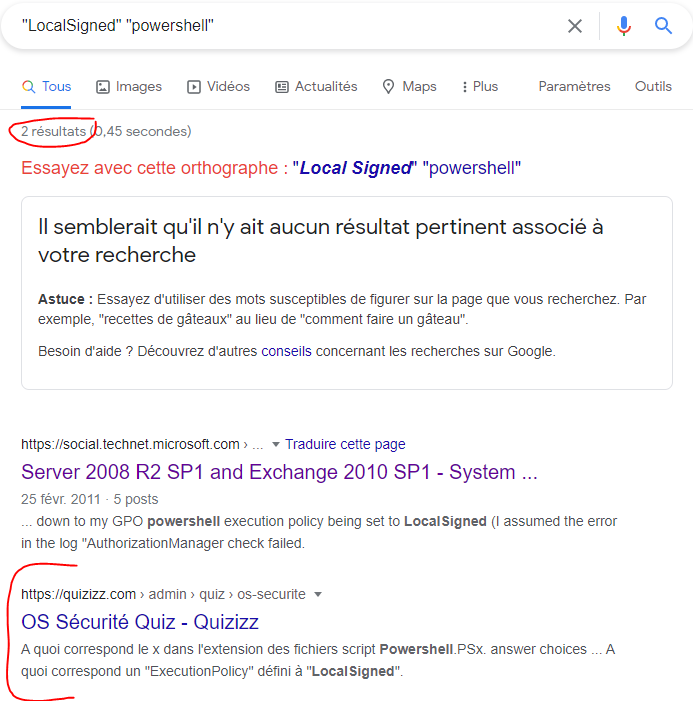
\includegraphics[width=0.65\linewidth]{images/LocalSigned.PNG} \end{example}
    \item Un script signé est également ?
    \begin{enumerate}
        \item Chiffré par clé symétrique
        \item Chiffré par clé asymétrique
        \item Chiffré par clé privée
        \item Chiffré par clé publique
        \item \textcolor{blue}{\textbf{Il n'est pas chiffré}}
    \end{enumerate}
    \item Veeam Backup \& Replication est conçu pour ?
    \begin{enumerate}
        \item \textcolor{blue}{\textbf{Les environnements virtualisés}}
        \item Les environnements physiques
        \item Les environnements Windows uniquement
        \item Les environnements Unix uniquement
        \item Aucune réponse n'est correcte
    \end{enumerate}
    \item Sur la machine à sauvegarder, Veeam Backup \& Replication a besoin d'installer ?
    \begin{enumerate}
        \item Un agent source-side
        \item Un agent target-side
        \item Un agent source-side et un agent target-side
        \item Un agent Veeam Backup Proxy
        \item \textcolor{blue}{\textbf{Aucune réponse n'est correcte}}
    \end{enumerate}
    \item L'élément Veeam Backup Repository de l'architecture Veeam B\&R sert à ?
    \begin{enumerate}
        \item Répondre aux requêtes de restauration
        \item Installer les agents sur les hôtes à sauvegarder
        \item \textcolor{blue}{\textbf{Sauvegarder les données de backup}}
        \item Administrer l'architecture Veeam B\&R
        \item Aucune réponse n'est correcte
    \end{enumerate}
    \item Lors d'un snapshot...
    \begin{enumerate}
        \item On fait une copie du disque dur et on la bloque en écriture
        \item \textcolor{blue}{\textbf{On bloque le disque dur en écriture et on enregistre les modifications sur un disque dur secondaire}}
        \item On bloque le disque dur en écriture pendant la création du backup
        \item Les modifications sont enregistrées sur le disque dur mais on attend la fin du backup pour les valider
        \item Aucune réponse n'est correcte
    \end{enumerate}
    \item Lors d'un Resersed Incremental Backup ?
    \begin{enumerate}
        \item \textcolor{blue}{\textbf{Le dernier point de sauvegarde est toujours complet}}
        \item Il est nécessaire de faire périodiquement une sauvegarde complète
        \item On ne peut effacer les sauvegardes intermédiaires qu'après une sauvegarde complète
        \item La politique de rétention varie en fonction de la périodicité de la sauvegarde complète
        \item Aucune réponse n'est correcte
    \end{enumerate}
    \item La déduplication est ?
    \begin{enumerate}
        \item Un système qui permet de faire une copie d'une machine, cela permet la redondance de machine et la haute disponibilité
        \item \textcolor{blue}{\textbf{Un système qui permet de vérifier si un bloc de données est déjà sauvegardé et ainsi éviter la redondance}}
        \item Un système qui permet de faire une copie des données sauvegardées. Cela permet la perte de données en cas de panne du serveur de stockage
        \item Un système qui virtualise une machine physique permettant ainsi de faire des tests sans toucher à la machine en production
        \item Aucune réponse n'est correcte
    \end{enumerate}
    \item Le monitoring ne permet pas la mesure ?
    \begin{enumerate}
        \item des performances
        \item de la disponibilité
        \item \textcolor{blue}{\textbf{de l'intégrité}}
        \item des modifications
        \item le monitoring permet la mesure de A, B, C, D
    \end{enumerate}
    \item SNMP est un protocole...
    \begin{enumerate}
        \item De surveillance de composants informatiques (ventilateur, sonde, ...)
        \item De contrôle à distance d'équipement informatique
        \item \textcolor{blue}{\textbf{De surveillance d'équipement réseau}}
        \item De surveillance d'application de type Java
        \item Les réponses A, B, C, D sont toutes correctes
    \end{enumerate}
    \item Un proxy Zabbix ?
    \begin{enumerate}
        \item \textcolor{blue}{\textbf{Peut collecter des données de performance et de disponibilité au nom du serveur Zabbix}}
        \item Est déployé sur des cibles de surveillance pour superviser activement les ressources locales et les applications, et envoyer les données collectées au serveur Zabbix
        \item Est le composant central auquel les agents envoient leur disponibilité, les informations d'intégrité et les statistiques
        \item Est un système de stockage base de données de toutes les informations de configuration ainsi que des données collectées par Zabbix
        \item Les réponses A, B, C, D sont toutes correctes
    \end{enumerate}
    \item Un élément Zabbix est ?
    \begin{enumerate}
        \item Un équipement sur le réseau que vous souhaitez surveiller, avec adresse IP/DNS
        \item Une expression logique qui définit un seuil de problème et qui est utilisée pour "évaluer" les données reçues dans les éléments
        \item Une occurence unique de quelque chose qui mérite l'attention, comme un changement d'état de déclenchement, un enregistrement automatique d'agent ou une découverte d'agent
        \item \textcolor{blue}{\textbf{Une donnée particulière que vous voulez recevoir d'un hôte, une métrique de données}}
        \item Aucune réponse n'est correcte
    \end{enumerate}
\end{enumerate}















\newpage \section{PAM - labo 3}





\begin{itemize}


\item Créer un utilisateur et supprimer son mdp: \texttt{adduser toto \&\& passwd -d toto}


\item \textbf{centos} - interdire la connexion des utilisateurs sans mdp en supprimant \textit{nullok}: \texttt{nano /etc/pam.d/system-auth}
\begin{example} \begin{verbatim}
auth sufficient pam_unix.so nullok try_first_pass
\end{verbatim} \end{example}


\item \textbf{debian} - modifier la politique de mot de passe:
\begin{itemize}
    \item \texttt{apt install libpam-cracklib}
    \item \texttt{nano /etc/pam.d/common-passwd} (ajouter cette ligne)
\begin{example} \begin{verbatim}
password required pam_cracklib.so retry=3 minlen=X difok=Y
\end{verbatim} \end{example}
\end{itemize}


\item \textbf{centos} - empêcher les utilisateurs de se connecter et afficher un message quand ils essaient:
\begin{itemize}
    \item \texttt{echo "Only root can login T\_T" > /etc/nologin}
    \item \texttt{nano /etc/pam.d/login}
\begin{example} \begin{verbatim}
account required pam_nologin.so
\end{verbatim} \end{example}
\end{itemize}


\item \textbf{debian} - idem sous debian:
\begin{itemize}
    \item \texttt{echo "Only root can login T\_T" > /etc/nologin}
    \item \texttt{nano /etc/pam.d/login}
\begin{example} \begin{verbatim}
auth requisite pam_nologin.so.
\end{verbatim} \end{example}
\end{itemize}


\item \textbf{debian} - ajouter une règle pour créer le dossier perso d'un utilisateur qui n'en a pas:
\begin{itemize}
    \item \texttt{nano /etc/pam.d/common-session}
\begin{example} \begin{verbatim}
session required pam_mkhomedir.so
\end{verbatim} \end{example}
    \item \texttt{su <user>}
\end{itemize}


\item \textbf{debian} - ajouter une règle pour que les changements de mdp des utilisateurs soient enregistrés:
\begin{itemize}
    \item \texttt{nano /etc/pam.d/common-password}
\begin{example} \begin{verbatim}
password required pam_pwhistory
\end{verbatim} \end{example}
\end{itemize}
\textbf{Remarque}: le changement est enregistré dans le dossier \texttt{/etc/security/opasswd}


\item \textbf{debian} - ajouter un délai de 10 sec après l'échec d'une tentative de connexion:
\begin{itemize}
    \item \texttt{nano /etc/pam/common-auth}
\begin{example} \begin{verbatim}
auth required pam_faildelay.so debug delay=10000000
\end{verbatim} \end{example}
\end{itemize}


\item \textbf{debian} - définir une plage horaire de connexion ssh pour un utilisateur:
\begin{itemize}
    \item \texttt{nano /etc/security/time.conf}
\begin{example} \begin{verbatim}
<service>;<terminal>;<utilisateur>;<time_range>
sshd;*;<user>;!Wd       # ssh interdit à l'utilisateur le WE
*;*;*;!Al1300-1400      # Wk = weekday, Wd = week-end, Al = any day
                        # 1300-1400 = 13-14h
\end{verbatim} \end{example}
\end{itemize}


\end{itemize}















\newpage \section{LDAP - labo 4}





\begin{itemize}


\item Installation/préparation:
\begin{example} \begin{verbatim}
# installer les paquets
yum -y install openldap compat-openldap openldap-clients openldap-servers \
    openldap-servers-sql openldap-devel

systemctl start slapd   # lance le service
systemctl enable slapd  # le service se lance au démarrage du système

netstat -antup | grep -i 389    # vérification: port ldap = 389

# -h <schéma_mdp> -s <nouveau_mdp>
slappasswd -h {SSHA} -s ldppassword > /etc/openldap/slapd.d/db.ldif
\end{verbatim} \end{example}


\item \texttt{cd /etc/openldap/slapd.d/}


\item Créer/modifier le fichier \texttt{db.ldif} pour modifier les variables \texttt{olcSuffix}, \texttt{olcRootDN} et \texttt{olcRootPW}:
\begin{example} \begin{verbatim}
# fichier à modifier in fine: ./cn=config/olcDatabase={2}hdb.ldif
dn: olcDatabase={2}hdb,cn=config
changetype: modify
replace: olcSuffix              # suffixe de la db (= nom de domaine)
olcSuffix: dc=greg,dc=local     # greg.local

dn: olcDatabase={2}hdb,cn=config
changetype: modify
replace: olcRootDN                      # root distinguished name (= root user)
olcRootDN: cn=ldapadm,dc=greg,dc=local  # root = ldapadm (nom standard ?)

dn: olcDatabase={2}hdb,cn=config
changetype: modify
replace: olcRootPW                                  # root's password
olcRootPW: {SSHA}d/thexcQUuSfe3rx3gRaEhHpNJ52N8D3   # hash obtenu avec "slappasswd"
\end{verbatim} \end{example}
\textbf{Remarque}: on ne fait pas les modifications directement dans le fichier car elles seraient perdues à chaque fois qu'on lance \texttt{ldapmodify}.


\item Envoyer les configurations au serveur ldap: \texttt{ldapmodify -Y EXTERNAL  -H ldapi:/// -f db.ldif}


\item Créer le fichier \texttt{monitor.ldif} pour modifier la variable \texttt{olcAccess}:
\begin{example} \begin{verbatim}
# fichier à modifier in fine: ./cn=config/olcDatabase={1}monitor.ldif
dn: olcDatabase={1}monitor,cn=config
changetype: modify
replace: olcAccess
olcAccess:
    {0}to * by dn.base="gidNumber=0+uidNumber=0,cn=peercred,cn=external,cn=auth"
    read by dn.base="cn=ldapadm,dc=greg,dc=local"
    read by * none
\end{verbatim} \end{example}
Syntaxe:
\begin{example} \begin{verbatim}
olcAccess: to [ressource]
    by [à qui] [type d'accès autorisé]
    by [à qui] [type d'accès autorisé]
\end{verbatim} \end{example}


\item Envoyer les configurations au serveur ldap: \texttt{ldapmodify -Y EXTERNAL  -H ldapi:/// -f monitor.ldif}


\item Copier la config de db et modifier le propriétaire:
\begin{example} \begin{itemize}
    \item \texttt{cp /usr/share/openldap-servers/DB\_CONFIG.example /var/lib/ldap/DB\_CONFIG}
    \item \texttt{chown ldap:ldap /var/lib/ldap/*}
\end{itemize} \end{example}


\item Ajouter les schémas ldap \textit{cosine} et \textit{nis} (= schémas des tables de la db ldap)\footnote{\url{https://ldap.com/understanding-ldap-schema/}}:
\begin{example} \begin{itemize}
    \item \texttt{ldapadd -Y EXTERNAL -H ldapi:/// -f /etc/openldap/schema/cosine.ldif}
    \item \texttt{ldapadd -Y EXTERNAL -H ldapi:/// -f /etc/openldap/schema/nis.ldif}
    \item \texttt{ldapadd -Y EXTERNAL -H ldapi:/// -f /etc/openldap/schema/inetorgperson.ldif}
\end{itemize} \end{example}


\item Créer le fichier \texttt{base.ldif} pour créer la base du directory ldap:
\begin{example} \begin{verbatim}
dn: dc=greg,dc=local
dc: greg
objectClass: top
objectClass: domain

dn: cn=ldapadm,dc=greg,dc=local
objectClass: organizationalRole
cn: ldapadm
description: LDAP Manager

dn: ou=People,dc=greg,dc=local
objectClass: organizationalUnit
ou: People

dn: ou=Group,dc=greg,dc=local
objectClass: organizationalUnit
ou: Group
\end{verbatim} \end{example}


\item Ajouter la base au domaine ldap: \texttt{ldapadd -x -W -D "cn=ldapadm,dc=greg,dc=local" -f base.ldif}


\item Créer le fichier \texttt{test01.ldif} pour créer un utilisateur \textit{test01}:
\begin{example} \begin{verbatim}
dn: uid=test01,ou=People,dc=greg,dc=local
objectClass: top
objectClass: account
objectClass: posixAccount
objectClass: shadowAccount
cn: test01
uid: test01
uidNumber: 9999
gidNumber: 100
homeDirectory: /home/test01
loginShell: /bin/bash
gecos: test01 [Admin (at) greg]
userPassword: {crypt}x
shadowLastChange: 17058
shadowMin: 0
shadowMax: 99999
shadowWarning: 7
\end{verbatim} \end{example}


\item Ajouter l'utilisateur: \texttt{ldapadd -x -W -D "cn=ldapadm,dc=greg,dc=local" -f test01.ldif}


\item Changer son mdp:
\begin{example} \begin{verbatim}
ldappasswd -s tttttt -W -D "cn=ldapadm,dc=greg,dc=local" \
    -x "uid=test01,ou=People,dc=greg,dc=local"
\end{verbatim} \end{example}


\item Vérification: \texttt{ldapsearch -x cn=test01 -b dc=greg,dc=local}


\item Ajouter le service ldap au parefeu:
\begin{example} \begin{itemize}
    \item \texttt{firewall-cmd --permanent --add-service=ldap}
    \item \texttt{firewall-cmd --reload}
\end{itemize} \end{example}


\item Modifier le fichier de log de ldap: \texttt{nano /etc/rsyslog.conf}
\begin{example} \begin{verbatim}
local4.* /var/log/ldap.log
\end{verbatim} \end{example}
\textbf{Remarque}: après, relancer le service: \texttt{systemctl restart rsyslog}


\item Configuration/vérification sur un client ldap:
\begin{example} \begin{verbatim}
# installation
yum install -y openldap-clients nss-pam-ldapd

# Enregistrer le client sur le serveur en SSO (SSO = single sign on)
authconfig --enableldap --enableldapauth --ldapserver=<ip_serveur_ldap> \
    --ldapbasedn="dc=greg,dc=local" --enablemkhomedir --update

systemctl restart nslcd     # redémarre le service ldap client

getent passwd test01        # vérification (1)
su test01                   # vérification (2)
\end{verbatim} \end{example}


\end{itemize}
















\newpage \section{LDAP - labo 5}





\begin{itemize}


\item Installation ldap sur debian:
\begin{example} \begin{itemize}
    \item \texttt{apt-get install slapd ldap-utils}
    \item \texttt{dpkg-reconfigure slapd}
\begin{example} \begin{verbatim}
Omettre la configuration OpenLDAP ?             Non
Nome de domaine DNS:                            henallux.local
Nom de l’organization ?                         Henallux
Mot de passe administrateur:                    tttttt
Confirmez le mot de passe:                      tttttt
Module de base de données à utiliser:           MDB
Supprimer la db lors de la purge du paquet ?    Oui
Faut-il déplacer l'ancienne base de données ?   Oui
\end{verbatim} \end{example}
\end{itemize} \end{example}


\item Modifier les variables d'environnement de base de ldap: \texttt{nano /etc/ldap/ldap.conf}
\begin{example} \begin{verbatim}
BASE    dc=henallux,dc=local
URI     ldap://<ip_machine>/    # on peut utiliser: 127.0.0.1
\end{verbatim} \end{example}


\item Vérification: \texttt{ldapsearch -xLLL}


\item Créer un répertoire \texttt{/root/ldap/conf} pour centraliser les fichiers de configuration:
\begin{example} \begin{itemize}
    \item \texttt{mkdir -p /root/ldap/conf}
    \item \texttt{cd /root/ldap/conf}
\end{itemize} \end{example}


\item Donner accès à l'admin à la config: \texttt{nano /root/ldap/conf/access-conf-admin.ldif}
\begin{example} \begin{verbatim}
dn: olcDatabase={0}config,cn=config
changeType: modify
add: olcAccess
olcAccess: to * by dn.exact=cn=admin,dc=henallux,dc=local manage by * break
\end{verbatim} \end{example}
Envoyer au serveur ldap: \texttt{ldapmodify -Y external -f access-conf-admin.ldif -H ldapi:///}
\begin{example} \begin{itemize}
    \item \texttt{-Y <mécanisme\_d\_authentification>} = spécifie la méthode d'authentification
    \item \texttt{-H ldapi:///} = \textcolor{red}{\textbf{???}}
\end{itemize} \end{example}


\item Interroger le serveur ldap avec la commande: \texttt{ldapsearch}
\begin{example}
    Exemple: \texttt{ldapsearch -D cn=admin,dc=henallux,dc=local -w tttttt}
    \begin{itemize}
        \item \texttt{-D <utilisateur>} = utilisateur qui va se connecter/faire la recherche
        \item \texttt{-w <mdp>} = mdp de l'utilisateur
        \item \texttt{-W} = demande le mdp après avoir lancé la commande
        \item \texttt{-y <fichier\_mdp>} = connexion avec le mdp contenu dans un fichier
        \item \texttt{-b <search\_base>} = endroit où on fait la recherche
        \item \texttt{-H ldap://<ip\_ldap>} = connexion à un serveur ldap distant
    \end{itemize}
\end{example}


\item Configurer les logs:
\begin{example} \begin{itemize}
    \item Configuration actuelle des logs: \texttt{ldapsearch -Y external -H ldapi:/// -b cn=config $\backslash$} \\
    \texttt{"(objectClass=olcGlobal)" olcLogLevel -LLL > log.ldif}
    \item Niveaux de logs:
\begin{example} \begin{verbatim}
-1   = enable all debugging
0    = no debugging
1    = trace function calls
2    = debug packet handling
4    = heavy trace debugging
8    = connection management
16   = print out packets sent and received
32   = search filter processing
64   = configuration file processing
128  = access control list processing
256  = stats log connections/operations/results
512  = stats log entries sent
1024 = print communication with shell backends
2048 = print entry parsing debugging
\end{verbatim} \end{example}
    \item Modifier le niveau de log: \texttt{nano log.ldif}
\begin{example} \begin{verbatim}
dn: cn=config
changetype: modify
replace: olcLogLevel
olcLogLevel: 256
\end{verbatim} \end{example}
    \item Envoyer la config au serveur ldap: \texttt{ldapmodify -Y EXTERNAL -H ldapi:/// -f log.ldif}
    \item Modifier le fichier de log de ldap: \texttt{nano /etc/rsyslog.conf}
\begin{example} \begin{verbatim}
LOCAL4.* -/var/log/slapd.log
\end{verbatim} \end{example}
    \item Redémarrer le service: \texttt{systemctl restart rsyslog}
\end{itemize} \end{example}


\item Les "overlays" (= modules/plugin supplémentaire)
\begin{example} \begin{itemize}
    \item Fichier d'installation d'overlay:
\begin{example} \begin{verbatim}
dn: cn=module,cn=config
cn: module
objectclass: olcModuleList
objectclass: top
olcmoduleload: <nom_module>.la
olcmodulepath: /usr/lib/ldap
\end{verbatim} \end{example}
    \item Envoyer le fichier au serveur ldap: \texttt{ldapadd -Y EXTERNAL -H ldapi:/// -f <fichier>.ldif}
    \item Fichier de conf d'overlay (ex: memberOf):
\begin{example} \begin{verbatim}
n: olcOverlay=memberof,olcDatabase={1}mdb,cn=config
changetype: add
objectClass: olcMemberOf
objectClass: olcOverlayConfig
objectClass: olcConfig
objectClass: top
olcOverlay: memberof
olcMemberOfDangling: ignore
olcMemberOfRefInt: TRUE
olcMemberOfGroupOC: groupOfNames
\end{verbatim} \end{example}
    \item Envoyer le fichier au serveur ldap: \texttt{ldapadd -Y EXTERNAL -H ldapi:/// -f <fichier>.ldif}
    \item Vérification:
\begin{example} \begin{itemize}
    \item \texttt{tree /etc/ldap/slapd.d/}
    \item \texttt{ldapsearch -QLLLY EXTERNAL -H ldapi:/// -b "cn=config" "Objectclass=olcmemberOf"}
\end{itemize} \end{example}
\end{itemize} \end{example}


\item Structure de l'annuaire ldap:
\begin{example} \begin{verbatim}
dc=henallux,dc=local
├── ou=group,dc=henallux,dc=local
│   ├── ou=techinfo,ou=group,dc=henallux,dc=local
│   └── ou=security,ou=group,dc=henallux,dc=local
│   ou=people,dc=henallux,dc=local
│   ├── ou=administration,ou=people,dc=henallux,dc=local
│   └── ou=profs,ou=people,dc=henallux,dc=local
├── ou=section,dc=henallux,dc=local
└── ou=system,dc=henallux,dc=local
\end{verbatim} \end{example}


\item Créer les OU (= organizational unit) (pas complet pour prendre moins de place):
\begin{example} \begin{verbatim}
dn: ou=people,dc=henallux,dc=local
ou: people
objectClass: organizationalUnit

dn: ou=section,dc=henallux,dc=local
ou: section
objectClass: organizationalUnit

dn: ou=group,dc=henallux,dc=local
ou: group
objectClass: organizationalUnit

dn: ou=system,dc=henallux,dc=local
ou: system
objectClass: organizationalUnit

dn: ou=administration,ou=people,dc=henallux,dc=local
ou: administration
objectClass: organizationalUnit
\end{verbatim} \end{example}
Envoyer au serveur: \texttt{ldapadd -cxWD cn=admin,dc=henallux,dc=local -f <fichier>.ldif}


\item Créer un utilisateur:
\begin{example} \begin{verbatim}
dn: uid=olivier,ou=administration,ou=people,dc=henallux,dc=local
objectclass: person
objectclass: organizationalPerson
objectclass: inetOrgPerson
uid: olivier
sn: olivier
givenName: Olivier
cn: Olivier
displayName: Olivier
userPassword: tttttt
mail: olivier@example.com
title: Admin
initials: N
\end{verbatim} \end{example}
Envoyer au serveur: \texttt{ldapadd -cxWD cn=admin,dc=henallux,dc=local -f <fichier>.ldif}


\item Il y a 2 types de groupes:
\begin{itemize}
    \item \texttt{posixgroup}, équivalent à un groupe unix
    \item \texttt{groupofnames}, équivalent à un groupe AD (problème: il doit toujours y avoir min 1 membre)
\end{itemize}


\item Créer un groupe:
\begin{example} \begin{verbatim}
dn: cn=secugrpa,ou=security,ou=group,dc=henallux,dc=local
cn: secugrpa
description: Securite Groupe A
objectClass: groupOfNames
member: cn=admin,dc=henallux,dc=local

dn: cn=secugrpb,ou=security,ou=group,dc=henallux,dc=local
cn: secugrpb
description: Securite Groupe B
objectClass: groupOfNames
member: cn=admin,dc=henallux,dc=local
\end{verbatim} \end{example}


\item Ajouter un membre à un groupe:
\begin{example} \begin{verbatim}
dn: cn=secugrpa,ou=security,ou=group,dc=henallux,dc=local
changetype: modify
add: member
member: uid=olivier,ou=administration,ou=people,dc=henallux,dc=local
\end{verbatim} \end{example}


\item Créer les comptes systèmes \texttt{viewer} et \texttt{writer} qui peuvent lire/écrire dans l'annuaire:
\begin{example} \begin{verbatim}
dn: cn=viewer,ou=system,dc=henallux,dc=local
objectClass: simpleSecurityObject
objectClass: organizationalRole
cn: viewer
description: LDAP viewer
userPassword: tttttt

dn: cn=writer,ou=system,dc=henallux,dc=local
objectClass: simpleSecurityObject
objectClass: organizationalRole
cn: writer
description: LDAP Writer
userPassword: tttttt
\end{verbatim} \end{example}


\item Afficher les ACL:
\begin{example} \begin{verbatim}
ldapsearch -xW -H ldap://localhost -D cn=admin,dc=henallux,dc=local \
    -b "cn=config" "olcDatabase={1}mdb" olcaccess
\end{verbatim} \end{example}


\item Modifier les ACL:
\begin{example} \begin{verbatim}
dn: olcDatabase={1}mdb,cn=config
changetype: modify
replace: olcAccess
olcAccess: to attrs=userPassword by self write
    by anonymous auth
    by dn="cn=writer,ou=system,dc=henallux,dc=local" write
    by dn="cn=viewer,ou=system,dc=henallux,dc=local" read
    by dn="cn=admin,dc=henallux,dc=local" write
    by * none
olcAccess: to dn.base="dc=henallux,dc=local" by users read
olcAccess: to * by self write
    by dn="cn=admin,dc=henallux,dc=local" write
    by * read by anonymous none
\end{verbatim} \end{example}
Envoyer au serveur: \texttt{ldapmodify -Q -Y EXTERNAL -H ldapi:/// -f acl.ldif}


\item Modifier une OU:
\begin{example} \begin{verbatim}
dn: ou=test,ou=people,dc=henallux,dc=local
changetype: modrdn
newrdn: ou=retest
deleteoldrdn: 1    
\end{verbatim} \end{example}
Envoyer au serveur: \texttt{ldapmodify -cxWD cn=admin,dc=henallux,dc=local -f <fichier>.ldif}


\item Déplacer une OU:
\begin{example} \begin{verbatim}
dn: ou=retest,ou=people,dc=henallux,dc=local
changetype: modrdn
newrdn: ou=retest
deleteoldrdn: 1
newsuperior: ou=techinfo,ou=group,dc=henallux,dc=local
\end{verbatim} \end{example}
Envoyer au serveur: \texttt{ldapmodify -cxWD cn=admin,dc=henallux,dc=local -f <fichier>.ldif}


\item Supprimer une OU (elle doit être vide) -- méthode 1:
\begin{example} \begin{verbatim}
dn: ou=retest,ou=techinfo,ou=group,dc=henallux,dc=local
changetype: delete
\end{verbatim} \end{example}
Envoyer au serveur: \texttt{ldapmodify -cxWD cn=admin,dc=henallux,dc=local -f <fichier>.ldif}


\item Supprimer une OU (elle doit être vide) -- méthode 2:
\begin{example} \begin{verbatim}
ou=retest,ou=techinfo,ou=group,dc=henallux,dc=local
\end{verbatim} \end{example}
Envoyer au serveur: \texttt{ldapdelete -cxWD cn=admin,dc=henallux,dc=local -f <fichier>.ldif}


\item Déplacer un utilisateur:
\begin{example} \begin{verbatim}
dn: uid=jean,ou=administration,ou=people,dc=henallux,dc=local
changetype: modrdn
newrdn: uid=jean
deleteoldrdn: 1
newsuperior: ou=profs,ou=people,dc=henallux,dc=local
\end{verbatim} \end{example}


\item Déplacer un groupe:
\begin{example} \begin{verbatim}
dn: cn=secugrpa,ou=security,ou=group,dc=henallux,dc=local
changetype: modrdn
newrdn: cn=secugrpa
deleteoldrdn: 1
newsuperior: ou=techinfo,ou=group,dc=henallux,dc=local
\end{verbatim} \end{example}


\item Renommer un utilisateur:
\begin{example} \begin{verbatim}
dn: uid=jean,ou=profs,ou=people,dc=henallux,dc=local
changetype: modrdn
newrdn: uid=pierre
deleteoldrdn: 1
\end{verbatim} \end{example}


\item Renommer un groupe:
\begin{example} \begin{verbatim}
dn: cn=secugrpa,ou=techinfo,ou=group,dc=henallux,dc=local
changetype: modrdn
newrdn: cn=tigrpb
deleteoldrdn: 1
\end{verbatim} \end{example}


\item Supprimer un utilisateur -- méthode 1:
\begin{example} \begin{verbatim}
dn: uid=pierre,ou=profs,ou=people,dc=henallux,dc=local
changetype: delete
\end{verbatim} \end{example}


\item Supprimer un utilisateur -- méthode 2 (directement en ligne de commande): \\
\begin{verbatim}
ldapdelete -cxWD cn=admin,dc=henallux,dc=local \
    uid=pierre,ou=profs,ou=people,dc=henallux,dc=local
\end{verbatim}


\item Supprimer un groupe -- méthode 1:
\begin{example} \begin{verbatim}
dn: cn=tigrpb,ou=techinfo,ou=group,dc=henallux,dc=local
changetype: delete
\end{verbatim} \end{example}


\item Supprimer un groupe -- méthode 2 (directement en ligne de commande):
\begin{verbatim}
ldapdelete -cxWD cn=admin,dc=henallux,dc=local \
    cn=tigrpb,ou=techinfo,ou=group,dc=henallux,dc=local    
\end{verbatim}


\item Ajouter un attribut à un utilisateur:
\begin{example} \begin{verbatim}
dn: uid=olivier,ou=administration,ou=people,dc=henallux,dc=local
changetype: modify
add: localityName
localityName: Namur
\end{verbatim} \end{example}


\item Modification d’attribut utilisateur:
\begin{example} \begin{verbatim}
dn: uid=carl,ou=administration,ou=people,dc=henallux,dc=local
changetype: modify
replace: UserPassword
UserPassword: rrrrrr
\end{verbatim} \end{example}


\item Modification de mot de passe utilisateur:
\begin{verbatim}
ldappasswd  -WS -H ldap://localhost
    -D "uid=olivier,ou=administration,ou=people,dc=henallux,dc=local"
\end{verbatim}


\item Modification d’attribut groupe:
\begin{example} \begin{verbatim}
dn: uid=olivier,ou=administration,ou=people,dc=henallux,dc=local
changetype: modify
replace: localityName
localityName: Bruxelles
\end{verbatim} \end{example}


\item Supprimer un attribut utilisateur:
\begin{example} \begin{verbatim}
dn: uid=olivier,ou=administration,ou=people,dc=henallux,dc=local
changetype: modify
delete: localityName
\end{verbatim} \end{example}


\item Supprimer un attribut groupe:
\begin{example} \begin{verbatim}
dn: cn=tigrpa,ou=techinfo,ou=group,dc=henallux,dc=local
changetype: modify
delete: member
member: uid=carl,ou=administration,ou=people,dc=henallux,dc=local
\end{verbatim} \end{example}


\end{itemize}





















\end{document}
